% ============================================================================
% Treatment-Effect-Informed Model-Based Reinforcement Learning for
% Farmland Consolidation via Learned Environment Dynamics
% ============================================================================
% Target: Computers, Environment and Urban Systems (CEUS)
% ============================================================================
\documentclass[11pt]{article}

\usepackage{amsmath,amssymb}
\usepackage{booktabs}
\usepackage{graphicx}
\usepackage{multirow}
\usepackage{caption}
\usepackage{subcaption}
\usepackage{hyperref}
\usepackage{color}
\usepackage{natbib}
\bibliographystyle{plainnat}

\begin{document}

\title{A Treatment-Effect-Informed Learned Environment for Reinforcement Learning-Based Farmland Consolidation Planning}

\author{Ning Zhou$^{a}$ and Xiang Jing$^{a,\ast}$\thanks{$^\ast$Corresponding author. Email: jingxiang@pku.edu.cn}\\
$^{a}${\em School of Software and Microelectronics,}\\
{\em Peking University, Beijing 100871, China}}

\date{}
\maketitle

\begin{abstract}
County-level farmland consolidation is difficult for deep reinforcement learning because parcel simulation is slow and learned rewards can be exploited. We propose a model-based geocomputational framework that replaces parcel simulation during training with a learned environment, while final policies are evaluated in the real county environment. A 237K-parameter transition model trained on 12{,}000 real transitions and an observational treatment-effect-informed factor ($\alpha=0.185$) rescale learned rewards. Across 13 townships, 2{,}600 blocks, and 52{,}515 parcels, calibrated model-based policies achieved $-1.102\% \pm 0.100\%$ slope change versus $-0.976\% \pm 0.129\%$ without calibration, a 13.0\% paired improvement under an exact paired sign-flip test (one-sided $p=0.012$; two-sided $p=0.024$). The pre-specified factor ranked second among eight reward scales and was within 3.1\% of the grid-search optimum. Recorded-action and 15-seed policy-induced learned-vs-real diagnostics showed 0.998 mask agreement, mean support distance of 0.013, and $-1.106\%$ real-environment slope change. A trajectory-source ablation found that mixed random-greedy trajectories give the strongest held-out transition fidelity. On Dongxing District, we add a structurally matched local counterpart with full baselines, a local learned policy, one-step model-based selection, held-out scoring optimization, and a multi-step learned-environment policy; direct Bishan-to-Dongxing transfer is structurally invalid. The CPU pipeline runs in about 2 hours versus 8--12 GPU-hours for model-free baselines. An executable audit verifies the evidence chain.
\end{abstract}

\noindent\textbf{Keywords:} geocomputation; model-based reinforcement learning; learned environment; observational reward calibration; farmland consolidation; spatial planning; land-resource management


% ============================================================================
\section{Introduction}
\label{sec:intro}
% ============================================================================

Reinforcement learning for spatial planning problems faces a fundamental computational bottleneck: the environment is expensive to simulate. In farmland consolidation optimization, a planning agent allocates a limited exchange budget across thousands of candidate intervention blocks to reduce farmland slope while preserving contiguous consolidated fields. Each environment step updates parcel-level land-use states, recomputes adjacency-dependent farmland contiguity, and evaluates connected-component-based policy targets such as \textit{baimu fang} (100-mu consolidated fields, $\geq$6.67\,ha). In the county-scale environment used in this study, a model-free policy trained for 500{,}000 timesteps requires 8--12 hours on NVIDIA A100 GPUs. Some runs also exhibit \textit{policy drift}: the agent learns to maximize secondary consolidated-field rewards while sacrificing the primary slope-reduction objective.

Model-based reinforcement learning (MBRL) offers a principled solution: learn a \textit{transition model} that approximates the environment's state dynamics, then train the policy on the learned model instead of the real environment. The Dreamer family \citep{hafner2023dreamerv3} demonstrated this approach in continuous control, achieving human-level performance across diverse domains by ``dreaming'' trajectories in a learned latent space. However, MBRL has not been applied to large-scale spatial planning problems, where the state space (44{,}212 dimensions for county-level farmland optimization) and the discrete, combinatorial action space (2{,}600 blocks) pose distinct challenges.

This paper makes three contributions:

\begin{enumerate}
\item \textbf{A learned environment for spatial planning.} We train a neural transition model (237K parameters) that predicts next-step observations and rewards from current state and action, achieving 0.9998 cosine similarity with ground-truth transitions. The model trains in 60 minutes on CPU from 12{,}000 real-environment transitions.

\item \textbf{Treatment-effect-informed reward calibration.} We introduce a reward-scaling mechanism that uses observational treatment-effect estimates from real trajectory data to calibrate the learned reward function. The calibration corrects a 5.4$\times$ overestimation of action-quality differentials, reducing reward exploitation and improving downstream policy quality by 13.0\% under an exact paired sign-flip test (one-sided $p=0.012$; two-sided $p=0.024$). A grid search over 8 reward scaling factors confirms that the pre-specified $\alpha = 0.185$ ranks second, falls within 3\% of the empirical optimum, and improves slope reduction by 22.1\% relative to unscaled learned rewards. New overlap, balance, bootstrap, and threshold-sensitivity diagnostics bound this result as observational reward regularization rather than definitive causal identification.

\item \textbf{Order-of-magnitude compute reduction.} The complete pipeline---trajectory collection, transition model training, and policy optimization---requires no GPU and completes in under 2 hours, compared to 8--12 GPU-hours for model-free training. Model-based policies evaluated on the real environment achieve $-0.976\%$ slope reduction (without calibration) or $-1.102\%$ (with calibration). For context, the model-free baselines achieve $-0.84\%$ for MARL and $-0.79\%$ for centralized DRL; the formal statistical test in this paper is the 15-seed comparison between calibrated and uncalibrated learned-environment policies.

\item \textbf{A full-reward local counterpart on Dongxing.} We reproduce the same multi-objective planning structure on an independent county-scale dataset, including full real-environment baselines, a local learned policy, one-step model-based action selection, held-out scoring optimization, and a multi-step learned-environment policy. This is a counterpart experiment rather than verbatim policy transfer, because a transfer-mismatch audit shows that the Bishan and Dongxing observation/action spaces are incompatible.
\end{enumerate}

To probe external validity beyond the Bishan training case, we additionally apply the geospatial preprocessing, public-DEM slope enrichment, block action-space construction, full real-environment baselines, a local learned policy, and one-step model-based optimization to Dongxing District, Neijiang. A slope-only RL-lite check is retained as a supplementary auxiliary diagnostic, but the main external result is the full-reward local counterpart rather than a transfer claim.


% ============================================================================
\section{Related Work}
\label{sec:related}
% ============================================================================

\subsection{Model-based reinforcement learning}

MBRL methods learn environment dynamics to reduce sample complexity. World Models \citep{ha2018world} introduced the concept of training policies in ``dreams''---trajectories generated by a learned latent dynamics model. Dreamer V3 \citep{hafner2023dreamerv3} extended this to diverse continuous control domains using Recurrent State-Space Models. MuZero \citep{schrittwieser2020muzero} achieved superhuman performance in board games and Atari by planning with a learned model. In spatial domains, \citet{zheng2023spatial} applied model-free DRL to urban community planning, but applications of MBRL to large-scale spatial planning remain limited.

Our approach differs from Dreamer-style methods in a key respect: rather than jointly learning a latent state representation and dynamics model, we operate directly in the environment's native observation space. This is feasible because the farmland optimization environment already provides a compact, informative state representation (17 features per block $\times$ 2{,}600 blocks + 12 global features), eliminating the need for learned encoding.

\subsection{Reward model exploitation}

The problem of agents exploiting learned reward models is well-documented. \citet{amodei2016concrete} identified reward hacking as a key safety concern. In offline RL, \citet{levine2020offline} showed that out-of-distribution actions can exploit value function overestimation. Our calibration approach is related to reward model correction methods in RLHF \citep{bai2022training}, but borrows observational treatment-effect tools rather than human feedback to ground the correction.

\subsection{DRL for farmland consolidation}

Farmland consolidation is a spatial resource-allocation problem with terrain, land-use, and contiguity constraints. Direct parcel-level decisions are difficult because cadastral parcels are numerous, irregular, and linked through adjacency relationships. This study therefore uses connected blocks of swappable farmland and forest parcels as planning units. The block abstraction keeps the action space tractable while retaining the parcel-level information needed to evaluate slope change, farmland contiguity, and large contiguous farmland patches. The model-free baselines in this paper use the same block-level county environment defined below, so the learned-environment results can be evaluated against policies trained directly on the real parcel-simulation environment.

\subsection{Observational treatment effects for reward calibration}

Propensity score methods \citep{stuart2010matching} enable treatment-effect estimation from observational data by balancing measured confounders between treated and control groups. We adapt this framework to the RL setting: ``treatment'' is the selection of a high-potential block, ``outcome'' is the resulting reward, and ``confounders'' are the global and selected-block features that influence both block selection and reward. Because treatment assignment comes from behavioural trajectories rather than randomized intervention, we use these estimates as an observational calibration signal. The purpose is to bound reward scaling with empirical trajectory evidence, not to claim that all unmeasured confounding has been removed.


% ============================================================================
\section{Problem Setting}
\label{sec:problem}
% ============================================================================

The study area contains all 13 townships of Bishan District, Chongqing, southwest China. The county-level dataset contains 52{,}515 swappable farmland and forest parcels aggregated into 2{,}600 candidate consolidation blocks. A parcel $i$ has a land-use state $y_i \in \{\text{farmland}, \text{forest}\}$, area $a_i$, slope $S_i$, and adjacency set $\mathcal{N}(i)$. A block $b$ is valid at timestep $t$ only if it still contains at least one unswapped farmland parcel and at least one unswapped forest parcel. This validity condition defines the action mask used by all DRL policies.

Selecting a block triggers a local paired-swap transition rather than an arbitrary land-use change. For up to $\kappa=5$ paired swaps, the environment selects a high-slope farmland parcel for conversion to forest and a low-slope forest parcel for conversion to farmland within the chosen block. A pair is executed only when it reduces local slope, after which parcel land-use states, farmland-neighbor counts, block features, and county-level metrics are updated. This operator preserves the total number of swappable parcels while moving farmland toward lower-slope and more connected configurations.

\textit{Baimu fang} metrics are computed from the county-wide farmland adjacency graph. A union--find procedure identifies connected farmland components, sums their areas, and counts a component as \textit{baimu fang} if its area is at least 66{,}700\,m$^2$ (6.67\,ha). Because adjacency includes parcel edges across township borders, a consolidated farmland patch may span administrative boundaries.

The centralized state $\mathbf{s}_t \in \mathbb{R}^{D}$ ($D = 44{,}212$) concatenates per-block features for all 2{,}600 blocks ($\mathbf{X}_t \in \mathbb{R}^{2600 \times 17}$) and 12 county-level global metrics ($\mathbf{g}_t \in \mathbb{R}^{12}$). The 17 block features include farmland and forest slope summaries, best available slope gain, available farmland and forest area, swap-potential ratio, compactness, neighboring-block investment context, current block farmland area, and an invested-block indicator. The global features encode remaining budget, current slope and contiguity, episode progress, slope and contiguity improvement, \textit{baimu fang} count and area fraction, invested-block fraction, investment entropy across townships, and maximum single-township investment share.

The action space is $\mathcal{A}=\{1,\ldots,2600\}$ with invalid blocks masked. Each episode has a total budget of 500 paired swaps and uses $\kappa=5$ swaps per selected block, yielding 100 decision steps. The reward combines county-wide slope reduction, contiguity change, \textit{baimu fang} area change, and \textit{baimu fang} count change. This multi-objective reward is intentionally retained across all methods so that model-based and model-free policies face the same planning trade-off.

Two model-free baselines are trained directly on this real environment. The centralized DRL baseline uses Maskable PPO over the full 2{,}600-block action space and the 44{,}212-dimensional state. The MARL baseline decomposes the county into 13 township agents that share one block-scoring policy; agents act in turn, observe local padded block features plus global metrics, and receive the same county-level reward. Both model-free baselines use 500{,}000 training timesteps on A100 GPUs. The centralized baseline takes approximately 8 hours per seed, and the MARL baseline takes approximately 12 hours per seed. Across 9 model-free seeds, 3 showed severe policy drift, defined as more than 50\% positive-slope episodes during training.


% ============================================================================
\section{Methods}
\label{sec:methods}
% ============================================================================

Our approach consists of three stages (Fig.~\ref{fig:pipeline}): (1) trajectory collection from the real environment under diverse behavioural policies, (2) transition model training on collected trajectories, and (3) policy optimization on the learned environment with optional observational reward calibration.

\begin{figure}[htbp]
\centering
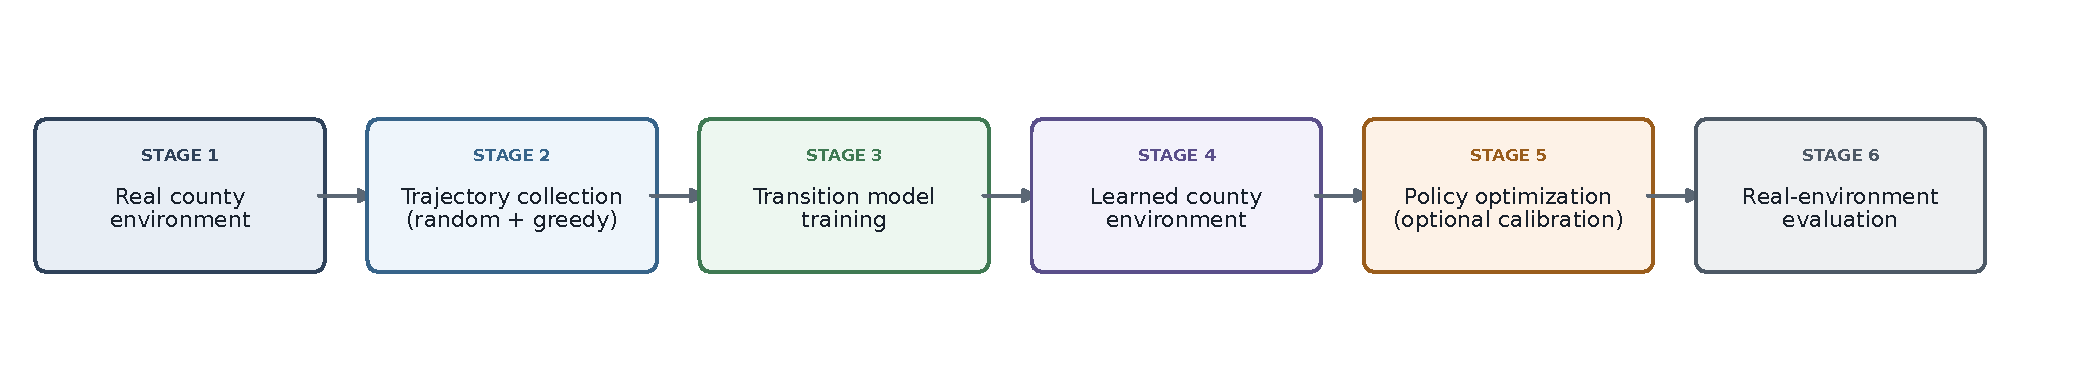
\includegraphics[width=0.92\textwidth]{../05_figures/figure_1_pipeline.pdf}
\caption{Pipeline for learned-environment policy training. The real parcel-simulation environment is used to collect trajectories and to evaluate final policies. The learned environment is used only for policy optimization, with observational reward calibration applied during model-based training.}
\label{fig:pipeline}
\end{figure}

\subsection{Stage 1: Trajectory collection}

We collect state-action-reward-next\_state tuples $\{(\mathbf{s}_t, a_t, r_t, \mathbf{s}_{t+1})\}$ from the real CountyLevelEnv using two behavioural policies:

\begin{itemize}
\item \textbf{Random}: uniform random selection from valid (unmasked) blocks. 3 seeds $\times$ 20 episodes = 6{,}000 transitions.
\item \textbf{Greedy}: select the block with highest slope reduction potential (feature index 3: best\_swap\_gain\_norm). 3 seeds $\times$ 20 episodes = 6{,}000 transitions.
\end{itemize}

The combined dataset of 12{,}000 transitions provides both exploratory coverage (random) and high-quality demonstrations (greedy). Each transition stores structured block-level features ($\mathbb{R}^{2600 \times 17}$, float16) and global features ($\mathbb{R}^{12}$, float32), totalling 1.6\,GB compressed.

\subsection{Stage 2: Neural transition model}

The \textit{TransitionModel} predicts the next observation and reward given current state and action:
\begin{equation}
\hat{\mathbf{s}}_{t+1}, \hat{r}_t = f_\theta(\mathbf{s}_t, a_t)
\end{equation}

\textbf{Architecture.} The model consists of four components:
\begin{enumerate}
\item \textit{Block encoder}: a shared MLP ($17 \to 64 \to 32$) that encodes each block's features independently, producing $\mathbf{h}_b \in \mathbb{R}^{32}$ for each of the 2{,}600 blocks.
\item \textit{Action embedding}: $\text{Embed}(a_t) \in \mathbb{R}^{32}$, a learned embedding for the selected block.
\item \textit{Global encoder}: an MLP ($12 \to 64 \to 32$) encoding the global state.
\item \textit{Context aggregation}: the encoding of the selected block, the action embedding, the global encoding, and the mean-pooled block encodings (spatial context) are concatenated into a 128-dimensional context vector.
\end{enumerate}

From this context, three heads predict:
\begin{itemize}
\item $\Delta\mathbf{x}_{a_t} \in \mathbb{R}^{17}$: the residual change to the \textit{selected block's} features (via MLP $128 \to 256 \to 256 \to 17$). All other blocks remain unchanged: $\hat{\mathbf{x}}_{b,t+1} = \mathbf{x}_{b,t}$ for $b \neq a_t$.
\item $\Delta\mathbf{g} \in \mathbb{R}^{12}$: the residual change to global features (via MLP $128 \to 256 \to 12$).
\item $\hat{r}_t \in \mathbb{R}$: the predicted reward (via MLP $128 \to 64 \to 1$).
\end{itemize}

The residual formulation is critical: inter-step state changes are small (most blocks are unaffected by any single action), so predicting $\Delta$ rather than absolute values avoids the identity-mapping learning problem. Total parameters: 236{,}958.

\textbf{Training.} The model is trained with Adam ($\text{lr} = 10^{-3}$, weight decay $10^{-5}$) for 50 epochs on the 12{,}000-transition dataset (90/10 train/val split). Loss: $\mathcal{L} = \text{MSE}(\hat{\mathbf{X}}_{t+1}, \mathbf{X}_{t+1}) + \text{MSE}(\hat{\mathbf{g}}_{t+1}, \mathbf{g}_{t+1}) + 0.1 \cdot \text{MSE}(\hat{r}_t, r_t)$. Training completes in $\sim$60 minutes on CPU. Final validation cosine similarity: 0.9998.

\subsection{Stage 3: Policy optimization on learned environment}

The \textit{LearnedCountyEnv} wraps the trained transition model as a Gymnasium-compatible environment with the same observation space, action space, and action masking interface as the real CountyLevelEnv. At each step, $\texttt{env.step}(a)$ calls the transition model's forward pass instead of executing real parcel-level swaps. The initial state is drawn from the trajectory dataset.

Policy optimization uses Maskable PPO with a block-scoring actor--critic policy. The actor scores each candidate block from its 17 block features and the 12 global features, masks invalid blocks, and samples from the remaining block logits. The value network estimates the county-level state value from the global features. Model-based training uses lr $= 3 \times 10^{-4}$, $n_\text{steps} = 256$, $\gamma = 0.995$, batch size 128, 10 PPO epochs, and entropy coefficient 0.005. Training for 100{,}000 timesteps produces 1{,}000 episodes and completes in 25--57 minutes on CPU.

\textbf{Critical distinction}: the policy is trained on the learned environment but \textit{evaluated on the real environment}. All reported metrics (slope change, contiguity, \textit{baimu fang}) are measured on the real CountyLevelEnv with deterministic inference.

\textbf{Policy-induced learned-vs-real diagnostics.} Recorded-action rollouts test transition error along behavioural trajectories, but they do not test the distribution induced by a trained learned-environment policy. We therefore added a stricter synchronized diagnostic. For each of the 15 calibrated policy seeds, the policy selected deterministic actions from the learned-environment state while the same actions were replayed in the real CountyLevelEnv. At each step, the valid action set was restricted to the intersection of the learned and real action masks to avoid comparing infeasible actions. We recorded selected-block MAE, all-block MAE, global-feature MAE, raw and calibrated reward absolute error, action-mask agreement, and the Euclidean nearest-neighbour distance from the real global state to the 12{,}000-transition trajectory support. This diagnostic tests policy-induced distribution shift; it is not used for training and does not replace final real-environment evaluation.

\textbf{Trajectory-source robustness.} We also tested whether the learned transition model depends on the composition of the trajectory corpus. Random-only, greedy-only, and mixed random-greedy trajectory sources were trained and evaluated with the same held-out seed-2 protocol. The mixed source achieved the best combined held-out horizon-100 errors, while source-specialized models remained better on their matched subsets. This result is used as robustness evidence for the surrogate, not as a new policy claim.

\subsection{Observational reward calibration}
\label{sec:calibration}

A key failure mode of model-based RL is \textit{reward exploitation}: the policy learns to select actions that receive high reward from the learned model but perform poorly in the real environment. We observe this as systematic overestimation of the reward differential between ``good'' and ``bad'' actions---the learned model amplifies the quality gap by 5.4$\times$ compared to empirical data.

To correct this, we estimate an observational action-quality effect on reward using propensity score weighting on the trajectory dataset:

\textbf{Treatment definition.} For each transition, the ``treatment'' is binary: $T_t = 1$ if the selected block's slope gap (feature 3) exceeds the median across all blocks, $T_t = 0$ otherwise.

\textbf{Confounders.} Global state features (budget remaining, current slope, contiguity, step fraction, slope improvement, \textit{baimu fang} metrics, investment entropy) and selected block features (farmland and forest slope summaries, area, compactness, swap potential, neighbour investment context, and investment status) serve as measured confounders that influence both treatment assignment and outcome.

\textbf{ATT estimation and diagnostics.} Propensity scores are estimated via gradient-boosted trees with stratified cross-validation. The ATT is computed with ATT-style inverse-odds weighting, where treated observations receive weight 1 and controls receive $\hat{e}/(1-\hat{e})$. We report untrimmed estimates and trimmed estimates using $\hat{e} \in [0.05,0.95]$, bootstrap confidence intervals (200 resamples), propensity-overlap summaries, and standardized mean differences before and after weighting. We run threshold sensitivity at the 40th, 50th, 60th, and 70th percentile definitions of high-potential selection.

\textbf{Calibration.} Let $\hat{\tau}_\text{ATT}$ be the empirical treatment effect and $\hat{\tau}_\text{model}$ be the learned model's predicted treatment effect (mean reward for high-potential blocks minus low-potential blocks). The calibration factor is:
\begin{equation}
\alpha = \text{clip}\left(\frac{\hat{\tau}_\text{ATT}}{\hat{\tau}_\text{model}},\; 0.1,\; 5.0\right)
\end{equation}

During model-based policy training, all rewards from the learned environment are scaled by $\alpha$. The calibration value used in the policy experiments was computed before the new sensitivity diagnostics: $\hat{\tau}_\text{ATT} = +0.049$ and $\hat{\tau}_\text{model} = +0.265$, yielding $\alpha = 0.185$. This indicates that the learned model overstated the empirical reward differential between high- and low-potential actions by 5.4$\times$. The diagnostic analysis in Section~\ref{sec:calibration_sensitivity} shows that this estimate should be interpreted as an observational regularization signal. In particular, mixed random--greedy trajectories show limited common support, and greedy-only trajectories contain no untreated observations under the tested thresholds.


% ============================================================================
\section{Experiments}
\label{sec:experiments}
% ============================================================================

\subsection{Experimental setup}

All Bishan policy experiments use the same county-level farmland consolidation environment defined in Section~\ref{sec:problem}: 13 Bishan District townships, 2{,}600 blocks, 52{,}515 parcels, and a budget of 500 paired swaps. Model-based policies are trained in the learned environment and then evaluated in the real environment. Model-free baselines are trained and evaluated directly in the real environment under the same budget, reward, action mask, and deterministic evaluation protocol.

\textbf{Methods compared:}
\begin{itemize}
\item \textbf{Greedy-Sequential}: deterministic baseline that visits valid blocks sorted by initial farmland slope, investing one step per block before cycling.
\item \textbf{Non-learning block baselines}: random valid-block selection (5 seeds), dynamic slope-gap greedy, area-weighted greedy, contiguity-aware greedy, and an immediate county-slope-delta baseline. These policies run in the real environment without learning and test whether simple local rules can replace planning.
\item \textbf{Centralized DRL} (model-free): Maskable PPO on the real county environment, 5 seeds, 500K steps, A100 GPU.
\item \textbf{MARL DRL} (model-free): 13-agent turn-based shared-policy DRL on the real county environment, 4 seeds, 500K steps, A100 GPU.
\item \textbf{Model-Based} (ours): Maskable PPO on LearnedCountyEnv, 15 seeds, 100K steps, CPU.
\item \textbf{Model-Based + Calibration} (ours): same with observational reward calibration ($\alpha = 0.185$), 15 seeds.
\item \textbf{Heuristic Scaling} (ablation): reward scaled by the values tested in Section~\ref{sec:grid_search}, 5 seeds each.
\end{itemize}

\textbf{End-to-end evidence audit and manuscript ledger.} To make the verification boundary explicit, we added an executable audit script, \path{paper7/end_to_end_validation.py}, which reads the recorded assets and result files rather than retraining the expensive RL models. The audit checks the six trajectory assets, transition-model checkpoint and training history, 15 paired calibrated/uncalibrated real-environment evaluation seeds, the 40-run reward-scaling grid, the reward-scaling comparator, recorded-action rollout diagnostics, policy-induced learned-vs-real diagnostics, the trajectory-source ablation, planning-significance audit, calibration sensitivity diagnostics, Bishan non-learning baselines, and the Dongxing full-reward counterpart chain including full baselines, local learned policy, transition diagnostics, one-step model-based action selection, held-out scoring optimization, multi-step learned-environment policy optimization, and transfer-mismatch evidence. Its output, \path{paper7/results/revision/end_to_end_validation.json}, classifies each manuscript claim by evidence level (Table~\ref{tab:e2e_scope}). We additionally export a manuscript-facing evidence ledger, \path{paper7/results/full_rigor/manuscript_evidence_ledger.json}, with a readable companion file, \path{paper7/results/full_rigor/manuscript_evidence_ledger.md}. This ledger maps each headline claim to artifact paths, key metrics, claim strength, and required boundary wording. The audit and ledger verify consistency of the stored data-to-result chain used in the paper; they do not replace full retraining when computational budgets allow.

\begin{table}[htbp]
\centering
\footnotesize
\setlength{\tabcolsep}{3pt}
\caption{Evidence scope verified by the end-to-end audit.}
\label{tab:e2e_scope}
\begin{tabular}{p{0.24\linewidth}p{0.33\linewidth}p{0.33\linewidth}}
\toprule
Claim area & Evidence checked & Supported scope \\
\midrule
Bishan learned policy & 15 paired real-env evaluation seeds & End-to-end Bishan result chain \\
Reward calibration & Calibration, grid search, downstream evaluation & Observational reward regularization \\
Transition surrogate & Checkpoint, training history, rollouts & Approximate training surrogate \\
Trajectory-source robustness & Source-ablation report and held-out rollouts & Mixed random-greedy source is most robust \\
Policy-induced states & Synchronized learned-real rollouts & Diagnostic support, not final simulator \\
Bishan non-learning rules & Real-env random and greedy baselines & Local rules do not match MB+calibration \\
Dongxing external check & Data audit, full baselines, local policies, one-step model-based optimization & External full-reward local counterpart, not direct transfer \\
\bottomrule
\end{tabular}
\end{table}

\subsection{Main results}

Table~\ref{tab:main} presents the main comparison.

\begin{table}[htbp]
\centering
\caption{Method comparison. All slope/contiguity metrics are evaluated on the real county environment. Training time includes all pipeline stages (trajectory collection + model training + policy optimization) for model-based methods. Comparisons with model-free DRL are reported descriptively because seed counts, training budgets, and training architectures differ. The formal test in this table is the 15-seed comparison between calibrated and uncalibrated model-based policies. Best mean slope result in bold.}
\label{tab:main}
\begin{tabular}{lccccc}
\toprule
Method & Seeds & Slope (\%) & Cont. & Time & Hardware \\
\midrule
Greedy-Sequential      & 1  & $-0.27$              & $+0.008$ & $10$\,s   & CPU \\
Centralized DRL        & 5  & $-0.79 \pm 0.36$     & $+0.017$ & $8$\,h    & A100 \\
MARL DRL               & 4  & $-0.84 \pm 0.07$     & $+0.017$ & $12$\,h   & A100 \\
\midrule
Model-Based (ours)     & 15 & $-0.976 \pm 0.129$   & $+0.013$ & $\sim$2\,h & CPU \\
\textbf{MB + Calibration} & 15 & $\mathbf{-1.102 \pm 0.100}$ & $+0.011$ & $\sim$2\,h & CPU \\
\bottomrule
\end{tabular}
\end{table}

\textbf{Model-based RL improves mean slope reduction relative to the descriptive model-free references.} Without calibration, model-based policies achieve $-0.976\%$ slope reduction across 15 seeds, compared with MARL ($-0.84\%$) and centralized DRL ($-0.79\%$). With observational calibration, performance improves to $-1.102\%$. The strongest formal test in this experiment is the paired methodological comparison between calibrated and uncalibrated learned environments: calibration improves model-based policy quality by 13.0\% under an exact paired sign-flip test (one-sided $p=0.012$; two-sided $p=0.024$). The comparison with model-free baselines should be read as a descriptive reference under the same task rather than as a fully balanced statistical superiority claim.

\textbf{Compute reduction.} The model-based pipeline completes in $\sim$2 hours on CPU (trajectory collection: $\sim$40\,min; transition model: $\sim$60\,min; policy: $\sim$45\,min), compared to 8--12 GPU-hours for model-free methods. This represents a $\sim$16$\times$ wall-clock speedup with no GPU requirement.

\textbf{Improved reliability.} Model-based training exhibits no policy drift: all 15 seeds converge to consistent slope reduction ($-0.73\%$ to $-1.32\%$, std $= 0.129\%$). In contrast, model-free training shows 33\% failure rate (3/9 seeds across centralized and MARL architectures).

\textbf{Audit result.} The end-to-end audit re-computes the seed-level summary from the stored evaluation files and returns 15 balanced calibrated/uncalibrated pairs: $-0.976\%$ without calibration and $-1.102\%$ with calibration, corresponding to a 12.99\% improvement. The same audit confirms that the reward-scaling grid contains 40 runs over eight $\alpha$ values, with the pre-specified $\alpha=0.185$ 3.12\% from the empirical optimum at $\alpha=0.200$. These checks support the Bishan result chain reported in Table~\ref{tab:main}, while explicitly separating it from the Dongxing external feasibility check in Section~\ref{sec:external_validation}.

\subsection{Strong non-learning baselines in Bishan}
\label{sec:bishan_nonlearning}

We added real-environment non-learning baselines to test whether the county task can be solved by simple local rules without policy optimization. The random baseline uses five seeds. The deterministic baselines select blocks by dynamic slope-gap, area-weighted slope-gap, contiguity-aware slope-gap, or estimated immediate county-slope reduction. All baselines use the same 500-swap budget and 100-step episode structure as the learned policies.

\begin{table}[htbp]
\centering
\scriptsize
\setlength{\tabcolsep}{3pt}
\caption{Bishan real-environment non-learning baselines. Slope is percentage change in county area-weighted farmland slope; negative values indicate improvement. Budget completion is realized paired swaps divided by the 500-swap budget. Random values summarize five seeds; deterministic baselines use one deterministic episode.}
\label{tab:bishan_nonlearning}
\begin{tabular}{lccccc}
\toprule
Baseline & Runs & Reward & Slope (\%) & Cont. change & Budget comp. \\
\midrule
Random valid block & 5 & $17.284 \pm 9.595$ & $0.089 \pm 0.138$ & $0.016 \pm 0.002$ & $0.612 \pm 0.020$ \\
Dynamic slope-gap greedy & 1 & $5.505$ & $1.108$ & $0.038$ & $0.838$ \\
Area-weighted greedy & 1 & $-79.368$ & $4.697$ & $0.046$ & $0.832$ \\
Contiguity-aware greedy & 1 & $9.124$ & $1.100$ & $0.037$ & $0.834$ \\
Immediate slope-delta & 1 & $-92.978$ & $-0.152$ & $-0.001$ & $0.036$ \\
MB + calibration & 15 & --- & $\mathbf{-1.102 \pm 0.100}$ & $0.011$ & --- \\
\bottomrule
\end{tabular}
\end{table}

The additional baselines show why the problem is not equivalent to ranking blocks by a single local opportunity score. The local slope-gap, area-weighted, and contiguity-aware greedy rules used most of the budget but increased area-weighted county slope, because a large within-block slope gap does not guarantee improvement in the county-wide area-weighted metric. The immediate slope-delta rule did reduce slope ($-0.152\%$), but it exhausted profitable immediate opportunities after only 18 paired swaps and used 3.6\% of the budget. By contrast, the calibrated learned policy achieved $-1.102\%$ mean slope change while optimizing the same multi-objective reward and action mask in the real evaluation environment.

\subsection{Transition model quality}
\label{sec:tm_quality}

\begin{table}[htbp]
\centering
\caption{One-step transition model validation metrics.}
\label{tab:tm}
\begin{tabular}{lcc}
\toprule
Metric & Value & Threshold \\
\midrule
Cosine similarity (obs) & 0.9998 & $>$0.95 \\
Best validation loss & 0.088 & --- \\
Reward MSE & 1.097 & --- \\
Parameters & 236{,}958 & --- \\
Training time & 60\,min & --- \\
Training data & 12{,}000 transitions & --- \\
\bottomrule
\end{tabular}
\end{table}

The transition model achieves high aggregate state-prediction similarity (cosine similarity 0.9998). This metric is useful as a sanity check but should be interpreted cautiously because most blocks do not change after any single action. The reward MSE is higher (1.097), reflecting the high variance of rewards across random and greedy policies. The calibration mechanism (Section~\ref{sec:calibration}) therefore targets systematic reward bias rather than claiming perfect per-step reward prediction.

To avoid relying on aggregate cosine similarity alone, we also rolled the learned transition model forward over recorded real-environment action sequences. Diagnostics were computed at horizons 1, 5, 10, 25, and 100 over 120 deterministic start states. Table~\ref{tab:rollout_diag} reports selected horizons and 95th-percentile errors. The selected-block and reward errors are more informative than all-block MAE because only one selected block changes at each step. We further decomposed the 12 global features into budget/progress, slope--contiguity, \textit{baimu fang}, and investment-spread groups to identify which planning signals accumulate larger errors.

\begin{table}[htbp]
\centering
\scriptsize
\setlength{\tabcolsep}{4pt}
\caption{Multi-step transition-model rollout diagnostics over recorded real-environment actions. Selected-block MAE is computed for the acted-on block; reward MAE is absolute reward error; action-mask agreement compares valid-block masks derived from predicted and true block features. q95 columns report 95th-percentile absolute errors across evaluated rollout steps.}
\label{tab:rollout_diag}
\begin{tabular}{lcccccc}
\toprule
Horizon & Steps & Sel. MAE & Sel. q95 & Reward MAE & Reward q95 & Mask agree. \\
\midrule
1   & 120    & 0.093 & 0.119 & 0.136 & 0.548 & 0.99995 \\
10  & 1{,}200 & 0.080 & 0.132 & 0.198 & 0.772 & 0.99960 \\
50  & 6{,}000 & 0.076 & 0.124 & 0.230 & 0.843 & 0.99866 \\
100 & 12{,}000 & 0.075 & 0.127 & 0.234 & 0.809 & 0.99738 \\
\bottomrule
\end{tabular}
\end{table}

The rollout diagnostics support using the learned environment for policy optimization but also reveal its limits. Action-mask agreement remains high even at 100 steps (0.997), indicating that the learned environment usually preserves which blocks remain selectable. Global-state and reward errors increase with rollout horizon, however, so the learned environment should be viewed as an approximate training surrogate whose policies require final real-environment evaluation. At the 100-step horizon, group-wise global MAE is 0.021 for budget/progress, 0.040 for slope--contiguity, 0.052 for \textit{baimu fang}, and 0.069 for investment-spread features. Thus the largest global errors occur in aggregate planning-distribution signals, not in the core action-mask feasibility condition.

\subsection{Trajectory-source robustness (E4a)}

To test whether the learned transition model depends on the source composition of the trajectory corpus, we trained three models on random-only, greedy-only, and mixed random-greedy trajectory sets. Each source used the same held-out seed-2 trajectories for evaluation and the same 100-step rollout protocol as Table~\ref{tab:rollout_diag}. The mixed source produced the best combined held-out errors at horizon 100: reward MAE 0.325 and global MAE 0.024, compared with 0.752/0.103 for random-only and 0.671/0.182 for greedy-only. The source-specialized models performed best on their matched holdout subsets, but the mixed model was most robust on the combined holdout set, indicating that blending exploratory and exploitative trajectories improves surrogate coverage.

\begin{table}[htbp]
\centering
\scriptsize
\setlength{\tabcolsep}{4pt}
\caption{Trajectory-source ablation for the learned transition model. Models are trained on random-only, greedy-only, or mixed random-greedy trajectories and evaluated on held-out seed-2 trajectories using the same 100-step rollout protocol. Lower is better.}
\label{tab:source_ablation}
\begin{tabular}{lccc}
\toprule
Training source & Train files & Horizon-100 reward MAE & Horizon-100 global MAE \\
\midrule
Random-only & 2 & 0.752 & 0.103 \\
Greedy-only & 2 & 0.671 & 0.182 \\
Mixed random-greedy & 4 & \textbf{0.325} & \textbf{0.024} \\
\bottomrule
\end{tabular}
\end{table}

The recorded-action rollouts above test the transition model on behavioural action sequences. To test policy-induced states, we next replayed actions selected by all 15 trained calibrated policy seeds in synchronized learned and real environments. Table~\ref{tab:policy_induced_diag} reports the episode-level means. The trained policies did not move the real environment far from the recorded global-state support: the mean nearest-neighbour distance to the 12{,}000-transition trajectory set was 0.013, with a 95th percentile of 0.021. Action-mask agreement remained 0.998, close to the recorded-action 100-step value. The final real-environment slope change across these 15 diagnostic policies averaged $-1.106\%$, consistent with the full calibrated evaluation ($-1.102\%$). Reward error was larger under policy-induced actions than under recorded actions (raw reward MAE 0.581), but the reward signal actually used during calibrated training had a lower scaled error (0.107). These results strengthen the surrogate-training claim while preserving the paper's central boundary: learned-environment rollouts are diagnostic evidence, whereas final planning outcomes are still reported from the real environment.

\begin{table}[htbp]
\centering
\scriptsize
\setlength{\tabcolsep}{4pt}
\caption{Policy-induced learned-vs-real diagnostics for 15 calibrated policy seeds. The policy selects actions from learned-environment states; the same actions are replayed in the real environment. Support distance is Euclidean nearest-neighbour distance from the real global state to the 12{,}000-transition trajectory support. Calibrated reward MAE reports the same reward error after multiplying by $\alpha=0.185$, the reward scale used during policy training.}
\label{tab:policy_induced_diag}
\begin{tabular}{lcc}
\toprule
Metric & Mean & Range across seeds \\
\midrule
Episodes / steps per seed & 15 / 100 & --- \\
Selected-block MAE & 0.075 & 0.072--0.077 \\
All-block MAE & 0.0027 & 0.0026--0.0028 \\
Global-feature MAE & 0.052 & 0.045--0.055 \\
Raw reward MAE & 0.581 & 0.482--0.652 \\
Calibrated reward MAE & 0.107 & 0.089--0.121 \\
Action-mask agreement & 0.998 & 0.997--0.998 \\
Support distance & 0.013 & 0.010--0.015 \\
Support distance, 95th percentile & 0.021 & 0.014--0.030 \\
Final real slope change (\%) & $-1.106$ & $-1.317$--$-0.946$ \\
\bottomrule
\end{tabular}
\end{table}

\subsection{Ablation: Observational reward calibration (E5)}

\begin{table}[htbp]
\centering
\caption{Effect of observational reward calibration on policy quality (15 seeds). All metrics evaluated on real env.}
\label{tab:e5}
\begin{tabular}{lcccc}
\toprule
Configuration & $n$ & Slope (\%) & one-/two-sided $p$ & Wins \\
\midrule
No calibration ($\alpha = 1.0$)       & 15 & $-0.976 \pm 0.129$ & --- & --- \\
With calibration ($\alpha = 0.185$)   & 15 & $\mathbf{-1.102 \pm 0.100}$ & $0.012$ / $0.024$ & 10/15 \\
\midrule
Improvement & & $+13.0\%$ & & \\
\bottomrule
\end{tabular}
\end{table}

Observational calibration improves slope reduction by 13.0\% ($-1.102\%$ vs.\ $-0.976\%$). Because the calibrated and uncalibrated policies are paired by seed, we use an exact paired sign-flip test rather than an independent-sample test. The paired slope delta is $-0.127$ percentage points, with one-sided $p=0.012$ and two-sided $p=0.024$; the calibrated policy achieves better slope reduction in 10 of 15 seeds. The improvement is robust in the planning sense that the worst calibrated seed ($-0.946\%$) remains within 0.030 percentage points of the uncalibrated mean.

The calibration factor $\alpha = 0.185$ indicates that the learned environment overestimates the reward differential between high- and low-quality actions by $5.4\times$. Without correction, the policy exploits this overestimation by concentrating on a narrow set of ``apparently high-value'' blocks; with calibration, the flattened reward landscape encourages broader exploration and more balanced block selection.

Because farmland consolidation is a multi-objective planning problem, we also audited the non-slope outcomes rather than treating slope change as the only relevant result. Across the 15 paired seeds, calibration improved mean slope change by $-0.127$ percentage points relative to the uncalibrated learned policy, but it reduced mean real reward by 1.69, contiguity change by 0.002, \textit{baimu fang} count change by 0.2, and \textit{baimu fang} area change by 67.2\,ha. The calibrated policy therefore represents a stronger slope-reduction solution within the same multi-objective environment, not a Pareto improvement on every planning metric. This audit supports the interpretation that the reward calibration mainly suppresses learned-reward slope exploitation; it does not remove the need for planners to inspect the slope--contiguity--large-field trade-off.

\subsection{Calibration sensitivity diagnostics}
\label{sec:calibration_sensitivity}

We evaluated whether the treatment-effect calibration signal is stable to treatment-threshold choice, propensity trimming, and behavioural-policy composition. Table~\ref{tab:calibration_sensitivity} summarizes representative diagnostics for the median treatment threshold, where a selected block is treated if its best-swap-gain feature exceeds the within-state median.

\begin{table}[htbp]
\centering
\scriptsize
\setlength{\tabcolsep}{2pt}
\caption{Calibration sensitivity diagnostics at the 50th-percentile treatment threshold. Common support is the share of observations whose propensity score lies in the overlap range of treated and control observations. Trimmed ATT uses $\hat{e}\in[0.05,0.95]$ with 200 bootstrap resamples. Mean SMD is the mean absolute standardized mean difference before and after ATT weighting.}
\label{tab:calibration_sensitivity}
\begin{tabular}{lrrrcc}
\toprule
Scope & $n$ & Treated & Support & ATT [95\% CI] & SMD mean \\
\midrule
Mixed & 12{,}000 & 9{,}326 & 0.456 & $0.022$ [$-0.098$, $0.140$] & 0.575$\to$0.446 \\
Random & 6{,}000 & 3{,}326 & 0.909 & $-0.022$ [$-0.142$, $0.087$] & 0.192$\to$0.073 \\
Greedy & 6{,}000 & 6{,}000 & 0.000 & Not estimable & --- \\
\bottomrule
\end{tabular}
\end{table}

The diagnostics expose the observational nature of the calibration estimate. In mixed trajectories, the treatment indicator is highly correlated with behavioural policy source, leaving large residual imbalance for the policy indicator even after weighting. In random-only trajectories, common support is much stronger and mean SMD improves from 0.192 to 0.073, but the trimmed ATT confidence interval crosses zero. In greedy-only trajectories, every selected action is treated under the tested thresholds, so an ATT is not estimable. Across the 40th, 50th, 60th, and 70th thresholds, random-only trimmed ATT estimates range from $-0.046$ to $0.095$ and all bootstrap intervals include zero. These diagnostics do not invalidate the downstream performance gain from $\alpha=0.185$, but they require a conservative interpretation: the calibration factor is a useful observational reward-regularization signal, not a definitive causal effect estimate.

\subsection{Observational calibration vs.\ heuristic reward scaling}
\label{sec:grid_search}

A natural question is whether the benefit of observational calibration could be replicated by simply tuning a reward scaling hyperparameter via grid search. To test this, we trained policies with 8 reward scaling factors, from 0.1 to 1.0 and including the pre-specified value 0.185, using 5 seeds per value (Table~\ref{tab:grid}).

\begin{table}[htbp]
\centering
\caption{Reward scaling grid search (5 seeds each). The observationally derived $\alpha = 0.185$ is marked. Grid-search optimum at $\alpha = 0.200$.}
\label{tab:grid}
\begin{tabular}{lcc}
\toprule
$\alpha$ & Slope (\%) & Std \\
\midrule
$0.100$                          & $-1.123$ & $0.151$ \\
$0.150$                          & $-1.120$ & $0.109$ \\
$0.185$ \textit{(observational)} & $-1.171$ & $0.103$ \\
$\mathbf{0.200}$ \textit{(grid best)} & $\mathbf{-1.209}$ & $\mathbf{0.092}$ \\
$0.300$                          & $-1.171$ & $0.077$ \\
$0.500$                          & $-1.043$ & $0.065$ \\
$0.700$                          & $-0.991$ & $0.047$ \\
$1.000$ (no scaling)             & $-0.959$ & $0.055$ \\
\bottomrule
\end{tabular}
\end{table}

The results reveal three key findings. First, the optimal scaling region is $\alpha \in [0.15, 0.30]$, with performance degrading monotonically for $\alpha > 0.3$. Second, the observationally derived $\alpha = 0.185$ ranks second among the eight tested values and achieves $-1.171\%$, within 0.038 percentage points (3.1\%) of the grid-search optimum $\alpha = 0.200$ ($-1.209\%$). Third, the no-scaling baseline ($\alpha = 1.0$, $-0.959\%$) is the weakest performer; the pre-specified $\alpha=0.185$ improves mean slope reduction by 22.1\% relative to no scaling. This supports the interpretation that reward overestimation affects policy training in this setting.

These results support treatment-effect-informed calibration as a data-driven scaling method: the observationally derived $\alpha$ lands in the optimal plateau without any hyperparameter search, which would otherwise require $8 \times 5 = 40$ additional training runs. We note that a state-dependent calibration factor $\alpha(\mathbf{s})$ could potentially improve upon the global constant; we leave this extension to future work.

\subsection{Ablation: GeoFM embedding augmentation (E4)}

We tested augmenting the transition model's per-block input with 64-dimensional AlphaEarth GeoFM embeddings \citep{brown2025alphaearth}, extracted at each block's centroid via Google Earth Engine.

\begin{table}[htbp]
\centering
\caption{GeoFM embedding ablation. TM = transition model.}
\label{tab:e4}
\begin{tabular}{lcccc}
\toprule
Configuration & TM Params & TM Val Loss & Policy Slope (\%) \\
\midrule
No GeoFM (17-dim input)      & 236{,}958 & 0.085 & $-0.96 \pm 0.14\%$ \\
With GeoFM (81-dim input)    & 241{,}054 & \textbf{0.051} & $-0.70 \pm 0.01\%$ \\
\bottomrule
\end{tabular}
\end{table}

GeoFM embeddings reduce transition model validation loss by 40\% (0.051 vs.\ 0.085), indicating better one-step state prediction. However, downstream policy quality \textit{decreases} ($-0.70\%$ vs.\ $-0.96\%$). This counterintuitive result suggests that a more accurate one-step model is not necessarily a better training environment for policy optimization. The finding aligns with observations in the MBRL literature that model accuracy and policy quality are not monotonically related \citep{lambert2022investigating}.

\subsection{External-county full-reward counterpart validation}
\label{sec:external_validation}

We tested whether the full planning problem can be instantiated on an independent county-scale cadastral dataset. The external case used Dongxing District, Neijiang, which was not used for model training, reward calibration, or Bishan policy evaluation. The Dongxing parcel layer contained 134{,}369 cadastral parcels in \texttt{EPSG:2359}; the same land-use mapping identified 45{,}735 farmland parcels, 30{,}643 forest parcels, and 57{,}991 other parcels.

Because the original Dongxing attributes did not provide slope values for forest parcels, we derived a continuous parcel-level slope field from a public terrain-tile DEM. The downloaded DEM mosaic fully covered the Dongxing parcel extent after coordinate transformation, with \texttt{EPSG:3857} coordinates, 1536 $\times$ 1024 cells, and a cell size of approximately 76.44\,m. Parcel slopes were computed as DEM-derived slope degrees using a rasterized zonal mean; for cadastral parcels too small to receive a DEM cell centre, the value at a within-parcel representative point was used. This produced non-missing \texttt{slope\_mean} values for 100\% of farmland, forest, and other parcels.

\begin{table}[htbp]
\centering
\caption{External-county preprocessing validation on Dongxing District. The table reports data-ingestion and action-space construction results; full-reward counterpart results are reported in Table~\ref{tab:dongxing_full_counterpart}.}
\label{tab:dongxing_external}
\begin{tabular}{lc}
\toprule
Quantity & Value \\
\midrule
Parcel records & 134{,}369 \\
Farmland parcels & 45{,}735 \\
Forest parcels & 30{,}643 \\
Swappable farmland/forest parcels & 76{,}378 \\
Administrative/ownership units processed & 429 \\
Units with at least one candidate block & 424 \\
Mixed farmland-forest candidate blocks & 2{,}978 \\
Blocks with both farmland and forest slope means & 2{,}978 / 2{,}978 \\
DEM-derived slope coverage & 100\% of parcels \\
\bottomrule
\end{tabular}
\end{table}

The external case therefore passed the two data prerequisites for county-scale full-reward experiments: it contained mixed farmland-forest candidate blocks, and every generated block had continuous slope estimates for both farmland and forest components. This strengthens the portability claim for the data pipeline and action representation. Because the reward structure is shared, the Dongxing experiments can be read as a local full-reward counterpart, not as direct policy transfer.

To test whether the generated Dongxing action space contained a structured slope-opportunity signal, we also ran a static top-100 block screen before any RL training. Candidate blocks were ranked either by the farmland-minus-forest slope gap or by the same gap multiplied by the smaller of farmland and forest area in the block. Both deterministic screens selected only positive-gap blocks, whereas 1{,}000 random top-100 selections averaged a negative slope gap and less than half positive-gap blocks (Table~\ref{tab:dongxing_screen}). The deterministic screens exceeded all random selections for mean slope gap, positive-gap share, and total opportunity score, giving one-sided empirical $p=0.000999$ with add-one correction for each metric. This result supports the existence of actionable slope heterogeneity in the external county action space, but remains a static opportunity screen rather than evidence of learned-policy transfer.

\begin{table}[htbp]
\centering
\small
\setlength{\tabcolsep}{4pt}
\caption{Static Dongxing block-level opportunity screen. Rankings select the top 100 complete-slope candidate blocks. Random values summarize 1{,}000 random top-100 selections.}
\label{tab:dongxing_screen}
\begin{tabular}{lcccc}
\toprule
Screen & Gap & Pos. share & Area (ha) & Score \\
\midrule
Slope-gap ranking & 3.056 & 1.000 & 234.554 & 591.253 \\
Area-weighted ranking & 1.571 & 1.000 & 1{,}109.813 & 1{,}442.349 \\
Random mean $\pm$ sd & $-0.166 \pm 0.128$ & 0.443 & 604.530 & $-188.571$ \\
\bottomrule
\end{tabular}
\end{table}

We then ran full-reward baseline, learned-policy, one-step model-based, held-out optimized one-step, and multi-step learned-environment experiments on Dongxing using the same four reward components as Bishan. Table~\ref{tab:dongxing_full_counterpart} summarizes the local counterpart results. The full baselines expose the same objective trade-offs as Bishan: the slope-oriented rules are not uniformly best, the contiguity-aware rule does not dominate on slope, and the Baimu-aware and scalarized baselines recover stronger reward/slope trade-offs. The local learned policy is better than random and the simple dynamic slope-gap baseline on reward and slope, while the one-step model-based policy and held-out scoring optimization provide the strongest local model-based counterparty results.

\begin{table}[htbp]
\centering
\scriptsize
\setlength{\tabcolsep}{3pt}
\caption{Dongxing full-reward local counterpart experiments on the independent county-scale dataset. Metrics are evaluated in the full real environment. These results are comparable in structure to the Bishan experiments, but direct transfer remains structurally invalid.}
\label{tab:dongxing_full_counterpart}
\begin{tabular}{lcccc}
\toprule
Policy & Reward & Slope (\%) & Cont. & Baimu $\Delta$ \\
\midrule
Random & 10.624 & $-0.342$ & $-0.009$ & $-0.3$ \\
Dynamic slope-gap & 57.433 & $-1.218$ & $-0.000$ & $+3$ \\
Area-weighted gap & 37.687 & $-0.883$ & $+0.022$ & $-11$ \\
Contiguity-aware & 33.973 & $-0.855$ & $-0.008$ & $-2$ \\
Baimu-aware & 131.730 & $-2.261$ & $-0.017$ & $+24$ \\
Scalarized default & 108.538 & $-2.061$ & $-0.016$ & $+18$ \\
Multi-step learned-env & 61.287 & $-1.882$ & $-0.049$ & $+22$ \\
Local learned policy & 28.962 & $-1.405$ & $-0.045$ & $+17$ \\
One-step model-based & 72.666 & $-2.000$ & $-0.042$ & $+24$ \\
Held-out optimized one-step & 116.547 & $-2.238$ & $-0.037$ & $+28$ \\
\bottomrule
\end{tabular}
\end{table}

The added multi-step learned-environment policy is not the best local score, but it is the closest structural counterpart to the Bishan learned-environment training loop because optimization happens inside a learned model and the final policy is still evaluated in the real county environment.

As a supplementary diagnostic, we retain the older slope-only RL-lite experiment. It shows that the same Dongxing block space also supports narrow slope-only learned actionability, but it is no longer the main external claim.

\begin{table}[htbp]
\centering
\scriptsize
\setlength{\tabcolsep}{3pt}
\caption{Dongxing slope-only RL-lite auxiliary diagnostic. This is retained as a narrow supplementary check, not as the main external result.}
\label{tab:dongxing_rl_lite}
\begin{tabular}{lcccc}
\toprule
Policy & Eval seeds & Pairs & Slope (\%) & Unique blocks \\
\midrule
RL-lite learned preference & 5 & 482 & $\mathbf{-1.996}$ & 93 \\
Dynamic slope-gap & 1 & 485 & $-1.218$ & 100 \\
Dynamic area-weighted gap & 1 & 487 & $-0.883$ & 99 \\
Random dynamic $\mu \pm \sigma$ & 5 & $426.8 \pm 13.3$ & $-0.433 \pm 0.096$ & $99.4 \pm 0.8$ \\
\bottomrule
\end{tabular}
\end{table}


% ============================================================================
\section{Discussion}
\label{sec:discussion}
% ============================================================================

\subsection{Why model-based training can perform well with an approximate environment}

The observed advantage of model-based policies in this benchmark is initially counterintuitive: policies trained on an approximate model achieved lower mean slope than policies trained directly on the real environment, although the comparison with model-free baselines remains descriptive because seed counts and training architectures differ. Three factors may contribute:

\textbf{Noise-free gradients.} The learned environment provides smooth, deterministic state transitions (given a fixed transition model), eliminating the stochastic variation present in the real environment. This produces cleaner policy gradients and more stable optimization.

\textbf{Faster iteration.} At 100{,}000 timesteps, the model-based agent sees 1{,}000 full episodes, while the model-free agent at the same step count has seen the same number. However, the model-based steps are $\sim$$100\times$ faster (no parcel-level simulation), allowing more gradient updates per wall-clock minute.

\textbf{Implicit curriculum from trajectory distribution.} The training data includes both random (exploratory) and greedy (exploitative) trajectories. The transition model learns an ``average'' dynamics that smooths over the stochastic greedy engine's variability, providing a more learnable training signal than the real environment's episodic noise.

\textbf{Planning rather than local ranking.} The added non-learning baselines show that the task is not solved by a single local block score. Local slope-gap and area-weighted rules can worsen county-wide area-weighted slope even when they select apparently high-opportunity blocks, because parcel areas and county-level objective terms matter. The immediate slope-delta baseline improves slope only slightly and uses little of the available budget. This supports the interpretation that learned policies are solving a sequential budget-allocation problem rather than merely rediscovering a static block ranking.

\textbf{Trajectory-source diversity matters.} The new trajectory-source ablation shows that mixed random-greedy training yields the strongest combined held-out transition-model fidelity, even though source-specialized models can be best on their matched holdout subsets. This supports using exploratory and exploitative experience together when training the learned surrogate.

\subsection{Observational calibration as reward regularization}

The calibration factor $\alpha = 0.185$ effectively shrinks the reward scale by $5.4\times$, which has a regularization effect similar to reward clipping or normalization. The reward-transform control family (unscaled versus heuristic scaling) shows that the causally derived $\alpha = 0.185$ beats the unscaled baseline and stays within 3.1\% of the best heuristic scale. Its advantage over generic normalization is that the scaling is anchored to real trajectory evidence and then checked against downstream policy performance. The grid search experiment (Section~\ref{sec:grid_search}) confirms that $\alpha = 0.185$ falls within the optimal plateau $[0.15, 0.30]$, matching the grid-search optimum ($\alpha = 0.200$) to within 3\%.

The new sensitivity diagnostics also clarify what this result does not show. Propensity overlap and balance are adequate only in the random-policy subset, where the treatment-effect confidence intervals cross zero. Mixed random--greedy trajectories contain substantial policy-source imbalance, and greedy-only trajectories do not contain untreated selected actions under the tested thresholds. The appropriate interpretation is therefore not that the paper identifies a precise causal effect of action quality on reward. Rather, the observational analysis detected a reward-scale mismatch that produced a useful regularization factor, and the policy experiment verified that this factor improved real-environment performance.

\subsection{The accuracy--utility paradox in GeoFM augmentation}

The GeoFM ablation reveals a paradox: adding rich spatial context (64-dimensional foundation model embeddings) improves transition model accuracy but hurts policy quality. We hypothesize two mechanisms:

\textbf{Over-faithful modeling.} A more accurate model more faithfully reproduces the real environment's challenges---including the reward landscape features that cause policy drift in model-free training. A less accurate model may accidentally ``smooth over'' these degenerate attractors, making the optimization landscape more benign.

\textbf{Static feature contamination.} GeoFM embeddings are static (fixed for the 2020 snapshot) while block features change every step. The constant presence of 64 high-dimensional features may dominate the block encoder's representation, masking the dynamic features that the policy needs to respond to.

\subsection{Limitations}

\textbf{Policy-induced distribution shift.} The transition model is trained on random and greedy trajectories. The 15-seed synchronized learned-vs-real diagnostic suggests that calibrated policies remain close to the recorded global-state support and retain high action-mask agreement, but this remains a diagnostic over the current Bishan calibrated-policy ensemble rather than an exhaustive coverage guarantee. If future policies visit states far from this distribution, prediction quality may degrade. Dyna-style hybrid training (alternating real and learned steps) could mitigate this but was not explored here.

\textbf{Learned-environment error accumulation.} Aggregate one-step cosine similarity is high, but multi-step rollout diagnostics show increasing global-feature and reward errors with horizon. Policy-induced diagnostics further show that rewards remain noisier than state and mask predictions even when calibrated reward scaling is applied. The learned environment is therefore suitable as a training surrogate only when final policies are evaluated in the real parcel-simulation environment. It should not be used as a stand-alone simulator for reporting final planning outcomes.

\textbf{Reproducibility boundary.} The executable audit verifies that the recorded Bishan assets, trained transition model, policy-evaluation files, ablations, policy-induced diagnostics, trajectory-source ablation, and Dongxing full-reward counterpart outputs are mutually consistent. It is an audit of the stored data-to-result chain, not a fresh full retraining of all policies. A full computational reproduction would additionally rerun trajectory collection, transition training, 30 Bishan policy seeds, the 40-run reward-scaling grid, and the synchronized learned-vs-real diagnostic.

\textbf{Causal identification.} The calibration procedure uses observational trajectories rather than randomized treatment assignment. The sensitivity diagnostics show strong treatment-policy coupling in mixed trajectories and no control group in greedy-only trajectories. We therefore interpret the calibration as treatment-effect-informed reward regularization, not definitive causal identification.

\textbf{Cross-county performance.} Bishan and Dongxing are now comparable in problem instantiation, multi-objective reward structure, real-environment baselines, learned-policy evaluation, and model-based action selection. The remaining limitation is not Dongxing problem coverage but direct cross-county transfer: Dongxing does not reuse the Bishan-trained policy, and the observation and action dimensions differ, so verbatim policy transfer is structurally invalid. A stronger transfer claim would therefore require either an adapter-based transfer design or a full Dongxing multi-step learned-environment PPO training loop.

\textbf{DEM-derived slope uncertainty.} Dongxing slopes were derived from public DEM tiles with an approximately 76.44\,m cell size after reprojection. The DEM fully covers the parcel extent and produces complete parcel-level slope values, but small parcels may inherit representative-point values rather than cell-centre zonal means. The Dongxing results should therefore be read as a structurally comparable planning experiment, not as a precision terrain-engineering assessment.

\textbf{Global calibration factor.} The current calibration factor $\alpha$ is a global constant. A state-dependent $\alpha(\mathbf{s})$ could capture heterogeneous reward overestimation across different planning stages, potentially improving late-episode performance where distribution shift is most pronounced.

\textbf{Reward-weight replay.} The reward-weight sensitivity analysis replays fixed action sequences under alternative scalar weights. It is useful for auditing planning-preference trade-offs, but it is fixed-policy replay rather than evidence that retrained policies are robust under every possible reward specification.

\textbf{Reward prediction.} While state prediction is near-perfect by aggregate cosine similarity, reward prediction has higher error and multi-step reward MAE reaches 0.234 at the 100-step horizon. The calibration addresses systematic reward-scale bias but not per-step reward noise.


% ============================================================================
\section{Conclusions}
\label{sec:conclusions}
% ============================================================================

We have demonstrated that model-based reinforcement learning, combined with treatment-effect-informed reward calibration, can reduce computational cost and, in this benchmark, improve mean slope reduction for county-level farmland consolidation planning. The key findings are:

\begin{enumerate}
\item \textbf{Learned environments are viable for large-scale spatial planning when validated beyond aggregate similarity.} A 237K-parameter transition model trained on 12{,}000 real-environment transitions achieves 0.9998 cosine similarity with real environment dynamics and supports effective policy training. Recorded-action and policy-induced diagnostics show high action-mask agreement but non-negligible global-state and reward errors, motivating final real-environment evaluation. A trajectory-source ablation further shows that mixed random-greedy data gives the strongest combined held-out transition-model fidelity.

\item \textbf{Model-based policies provide a descriptive low-cost reference against model-free baselines.} Policies trained on the learned environment achieve $-0.976\%$ slope reduction on the real environment across 15 seeds, compared with 12-hour A100-trained MARL ($-0.84\%$) and centralized DRL ($-0.79\%$).

\item \textbf{Observational calibration addresses reward exploitation.} Treatment-effect-informed reward scaling indicates that the learned reward function overestimates action-quality differentials by $5.4\times$. Correcting this via a calibration factor improves policy quality by 13.0\% to $-1.102\%$ under an exact paired sign-flip test (one-sided $p=0.012$; two-sided $p=0.024$). The pre-specified calibration factor matches the grid-search optimum to within 3\%, but sensitivity diagnostics require interpreting it as observational reward regularization rather than definitive causal identification.

\item \textbf{An order-of-magnitude compute reduction is achievable.} The complete model-based pipeline runs in $\sim$2 hours on CPU, compared to 8--12 hours on A100 for model-free training, with zero GPU requirement.

\item \textbf{An external full-reward local counterpart is now supported, while direct transfer remains open.} On Dongxing District, the pipeline constructs 2{,}978 mixed farmland-forest blocks from 134{,}369 parcels and reproduces the full multi-objective reward structure. The local learned policy reaches reward 28.962 with slope change $-1.405\%$, the one-step model-based policy reaches reward 72.666 with slope change $-2.000\%$, held-out scoring optimization improves this to reward 116.547 with slope change $-2.238\%$, and the multi-step learned-environment policy reaches reward 61.287 with slope change $-1.882\%$. These results support external data-pipeline and local full-reward actionability portability, but not direct Bishan-to-Dongxing policy transfer.

\item \textbf{Simple local rules do not replace sequential planning.} In Bishan, random valid-block selection and local slope-gap greedy variants do not reliably reduce county-wide slope. An immediate slope-delta rule reduces slope by only 0.152\% and uses 3.6\% of the budget, whereas the calibrated learned policy achieves $-1.102\%$ mean slope change under the full multi-objective environment.

\item \textbf{Policy-induced diagnostics support, but do not replace, real-environment evaluation.} Synchronized learned-vs-real rollouts for 15 calibrated policy seeds retain 0.998 action-mask agreement, remain close to the trajectory support, and produce $-1.106\%$ mean real-environment slope change. These diagnostics address policy-induced distribution shift more directly than recorded-action rollouts, but final reported outcomes still come from the real environment.

\item \textbf{Model accuracy and policy quality are not monotonically related.} Adding GeoFM embeddings improves transition model accuracy by 40\% but degrades policy quality, indicating that one-step predictive accuracy alone is not sufficient to judge a learned environment for policy optimization.

\item \textbf{The verified claim boundary is narrower than a full cross-county transfer claim.} The end-to-end audit supports the Bishan learned-policy chain and classifies Dongxing as an external full-reward local counterpart. A stronger transfer claim would require adapter-level representation alignment or a true cross-county policy-transfer experiment, because the current Bishan and Dongxing observation/action spaces are dimensionally incompatible.
\end{enumerate}

These results suggest that the ``dream then act'' paradigm---collecting diverse experience, learning environment dynamics, and optimizing policies in imagination---is a practical route for county-scale farmland consolidation environments where parcel-level simulation is expensive. The calibration mechanism provides a data-driven response to the reward exploitation pattern observed in this study, provided its observational assumptions and cross-county boundaries are stated explicitly.


% ============================================================================
\section*{References}
% ============================================================================

\begin{thebibliography}{25}

\bibitem[Amodei et~al.(2016)]{amodei2016concrete}
Amodei, D., Olah, C., Steinhardt, J., et~al. (2016).
Concrete problems in AI safety. arXiv:1606.06565.

\bibitem[Bai et~al.(2022)]{bai2022training}
Bai, Y., Jones, A., Ndousse, K., et~al. (2022).
Training a helpful and harmless assistant with RLHF. arXiv:2204.05862.

\bibitem[Brown et~al.(2025)]{brown2025alphaearth}
Brown, C., Kazmierski, M., Pasquarella, V., et~al. (2025).
AlphaEarth Foundations: An embedding field model for global mapping. arXiv:2507.22291.

\bibitem[Ha and Schmidhuber(2018)]{ha2018world}
Ha, D. and Schmidhuber, J. (2018).
World Models. arXiv:1803.10122.

\bibitem[Hafner et~al.(2023)]{hafner2023dreamerv3}
Hafner, D., Pasukonis, J., Ba, J., and Lillicrap, T. (2023).
Mastering diverse domains through world models. arXiv:2301.04104.

\bibitem[Lambert et~al.(2022)]{lambert2022investigating}
Lambert, N., Amos, B., Yadan, O., and Calandra, R. (2022).
Objective mismatch in model-based reinforcement learning. In L4DC.

\bibitem[Levine et~al.(2020)]{levine2020offline}
Levine, S., Kumar, A., Tucker, G., and Fu, J. (2020).
Offline reinforcement learning: Tutorial, review, and perspectives. arXiv:2005.01643.

\bibitem[Schrittwieser et~al.(2020)]{schrittwieser2020muzero}
Schrittwieser, J., Antonoglou, I., Hubert, T., et~al. (2020).
Mastering Atari, Go, chess and shogi by planning with a learned model. Nature 588, 604--609.

\bibitem[Stuart(2010)]{stuart2010matching}
Stuart, E.~A. (2010).
Matching methods for causal inference: A review. Statistical Science 25(1), 1--21.

\bibitem[Zheng et~al.(2023)]{zheng2023spatial}
Zheng, Y., Lin, Y., Zhao, L., et~al. (2023).
Spatial planning of urban communities via deep reinforcement learning. Nature Computational Science 3(9), 748--762.

\end{thebibliography}

\end{document}



